\documentclass[12pt]{article}
\usepackage{amsmath}
\usepackage{mathtools}
\usepackage{bigints}
\usepackage{parskip}
\usepackage{amssymb}
\usepackage{relsize}
\usepackage{fullpage}
% \DeclareMathSizes{12}{17.28}{9}{7} % (a)

\DeclareMathSizes{12}{17.28}{12}{12} % (a)


\usepackage{hyperref}



	\addtolength{\topmargin}{-.5in}
	\addtolength{\textheight}{1.75in}



    \newenvironment{myindentpar}[1]%
     {\begin{list}{}%
             {\setlength{\leftmargin}{#1}}%
             \item[]%
     }
     {\end{list}}

\begin{document}
\title{College Algebra: Module 4 What You Need To Know}
\date{2-12-15}
\author{}
\maketitle


\section{Linear Inequalities in One Variable (Section 1.2)}

In this section we learn how to solve linear inequalities. In order to do that we need to learn the notation used to represent intervals. The table below summarizes how to represent intervals using three different types of notation:

\begin{enumerate}

\item Interval Notation
\item Number Line Notation
\item Set-Builder Notation

\end{enumerate}

It is important to be able to represent our answers in either of the three notations and be able to convert between the different notations if needed.

\centerline{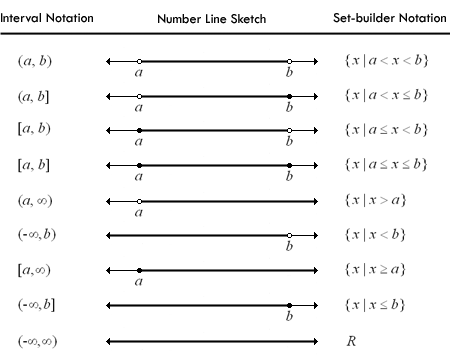
\includegraphics[scale = 0.8]{SetInterval.png}}

\textbf{Multiplicative Property of Inequalities}

\begin{enumerate}

\item If $a < b$ and $c > 0 \implies ac < bc$ 
\item If $a < b$ and $c < 0 \implies ac > bc$

\end{enumerate}

\newpage

\textbf{Division Property of Inequalities}

\begin{enumerate}

\item If $a < b$ and $c > 0 \implies \dfrac{a}{c} < \dfrac{b}{c}$ 
\item If $a < b$ and $c < 0 \implies \dfrac{a}{c} > \dfrac{b}{c}$

\end{enumerate}

\textbf{Note:} The same exact multiplicative and division property applies if the inequalities being used are less than or equal to ($\leq$) or greater than or equal to ($\geq$) inequalities. To summarize, the previous two properties just tell you one simple thing: \textbf{flip the inequality sign whenever you multiply or divide by a negative number!}

\textbf{Compound Inequalities:}

\textit{Compound Inequalities} are inequalities where the solution is the union of 2 or more intervals. In Mathematics, we use have a symbol which represents the \textbf{union} between two intervals. That symbol is given by $\cup$. Just remember: UNION $ = \cup$. As an example, the union between the two sets $(-5, 0]$ and $(3, 10)$ can be written as $(-5,0] \cup (3, 10)$.

\section{Absolute Value Equations and Inequalities (Section 1.3)}


\textbf{Def:} The \textit{absolute value} of a number $x$ is denoted by $|x|$ and defined to be 

\abovedisplayskip=0pt\relax
\[
\lvert x \rvert =
\begin{cases}
x & \text{if } x \geq0\\
-x& \text{if } x<0
\end{cases}
\]

\subsection{Absolute Value Equations}

\textbf{Property 1:} If $|x| = a \implies x = a$ or $x = -a$

\textbf{Propert 2:} $|x \cdot y| = |x| \cdot |y|$

\subsection{Absolute Value Inequalities}

\textbf{Note:} Remember the following two properties when solving absolute value inequalities:

\begin{itemize}
\item $|x| < a \implies -a < x < a$ 
\item $|x| > a \implies x<-a$ or  $x>a$ 
\end{itemize}

The same exact rule above applies if the inequalites are less than or equal to ($\leq$) or greater than or equal to ($\geq$) and just for reference I am giving those rules below:

\begin{itemize}
\item $|x| \leq a \implies -a \leq x \leq a$
\item $|x| \geq a \implies x\leq -a$ or  $x\geq a$
\end{itemize}













\end{document}